\chapter{Diseño e implementación} % Main chapter title

\label{Chapter3} % Change X to a consecutive number; for referencing this chapter elsewhere, use \ref{ChapterX}

\definecolor{mygreen}{rgb}{0,0.6,0}
\definecolor{mygray}{rgb}{0.5,0.5,0.5}
\definecolor{mymauve}{rgb}{0.58,0,0.82}

%%%%%%%%%%%%%%%%%%%%%%%%%%%%%%%%%%%%%%%%%%%%%%%%%%%%%%%%%%%%%%%%%%%%%%%%%%%%%
% parámetros para configurar el formato del código en los entornos lstlisting
%%%%%%%%%%%%%%%%%%%%%%%%%%%%%%%%%%%%%%%%%%%%%%%%%%%%%%%%%%%%%%%%%%%%%%%%%%%%%
\lstset{ %
  backgroundcolor=\color{white},   % choose the background color; you must add \usepackage{color} or \usepackage{xcolor}
  basicstyle=\footnotesize,        % the size of the fonts that are used for the code
  breakatwhitespace=false,         % sets if automatic breaks should only happen at whitespace
  breaklines=true,                 % sets automatic line breaking
  captionpos=b,                    % sets the caption-position to bottom
  commentstyle=\color{mygreen},    % comment style
  deletekeywords={...},            % if you want to delete keywords from the given language
  %escapeinside={\%*}{*)},         % if you want to add LaTeX within your code
  %extendedchars=true,             % lets you use non-ASCII characters; for 8-bits encodings only, does not work with UTF-8
  %frame=single,	                 % adds a frame around the code
  keepspaces=true,                 % keeps spaces in text, useful for keeping indentation of code (possibly needs columns=flexible)
  keywordstyle=\color{blue},       % keyword style
  language=[ANSI]C,                % the language of the code
  %otherkeywords={*,...},          % if you want to add more keywords to the set
  numbers=left,                    % where to put the line-numbers; possible values are (none, left, right)
  numbersep=5pt,                   % how far the line-numbers are from the code
  numberstyle=\tiny\color{mygray}, % the style that is used for the line-numbers
  rulecolor=\color{black},         % if not set, the frame-color may be changed on line-breaks within not-black text (e.g. comments (green here))
  showspaces=false,                % show spaces everywhere adding particular underscores; it overrides 'showstringspaces'
  showstringspaces=false,          % underline spaces within strings only
  showtabs=false,                  % show tabs within strings adding particular underscores
  stepnumber=1,                    % the step between two line-numbers. If it's 1, each line will be numbered
  stringstyle=\color{mymauve},     % string literal style
  tabsize=2,	                     % sets default tabsize to 2 spaces
  title=\lstname,                  % show the filename of files included with \lstinputlisting; also try caption instead of title
  morecomment=[s]{/*}{*/}
}


%----------------------------------------------------------------------------------------

Este capítulo describe el diseño y la implementación de cada uno de los componentes que conforman el sistema.
Se explican las decisiones de diseño, los flujos de trabajo y los aspectos técnicos involucrados en la construcción de cada módulo principal.

%---------------------------------------------------------------------------------------
\section{Arquitectura del sistema}

El sistema está diseñado para permitir la implementación y operación de un chatbot mediante un enfoque de recuperación aumentada por generación. 
Se implementó una arquitectura modular, basada en servicios en la nube, que facilita la escalabilidad y el mantenimiento del chatbot, y permite 
una actualización ágil de los componentes y una experiencia optimizada para los usuarios finales. En la figura \ref{fig:architecture} se ilustra
el diagrama de arquitectura, donde se observan la totalidad de los componentes que conforman el sistema.

En primer lugar, los usuarios interactúan con el chatbot a través de una interfaz gráfica (desarrollada con NextUI y deployada en Azure Static Web App), 
donde consultan por la información deseada. Estas consultas son luego transferidas al servidor (Azure App Service) a través de una API desarrollada 
con la librería FastAPI. Una vez allí, se realiza un proceso de búsqueda por similitud que toma la solicitud del usuario y la compara con la información
disponible en la base de datos (Azure AI Search), con el objetivo de identificar aquellos fragmentos más relevantes. Previamente, un administrador
debe haber cargado aquellos documentos que conforman la base de conocimiento del chatbot en un repositorio de GitHub, tras lo cual se ejecuta una 
automatización que los procesa y los envía a la base de datos.

Finalmente, la consulta del usuario y los fragmentos relevantes se envían al modelo LLM (desplegado en el servicio Azure OpenAI), que genera una 
respuesta contextualizada, que es devuelta a la interfaz gráfica para ser presentada al usuario.

Además, se incluye una pequeña base de datos adicional (Azure Table Storage) que se utiliza para guardar el feedback de los usuarios, 
para así obtener métricas del desempeño del chatbot.  

\vspace{30mm}

\begin{figure}[ht]
	\centering
	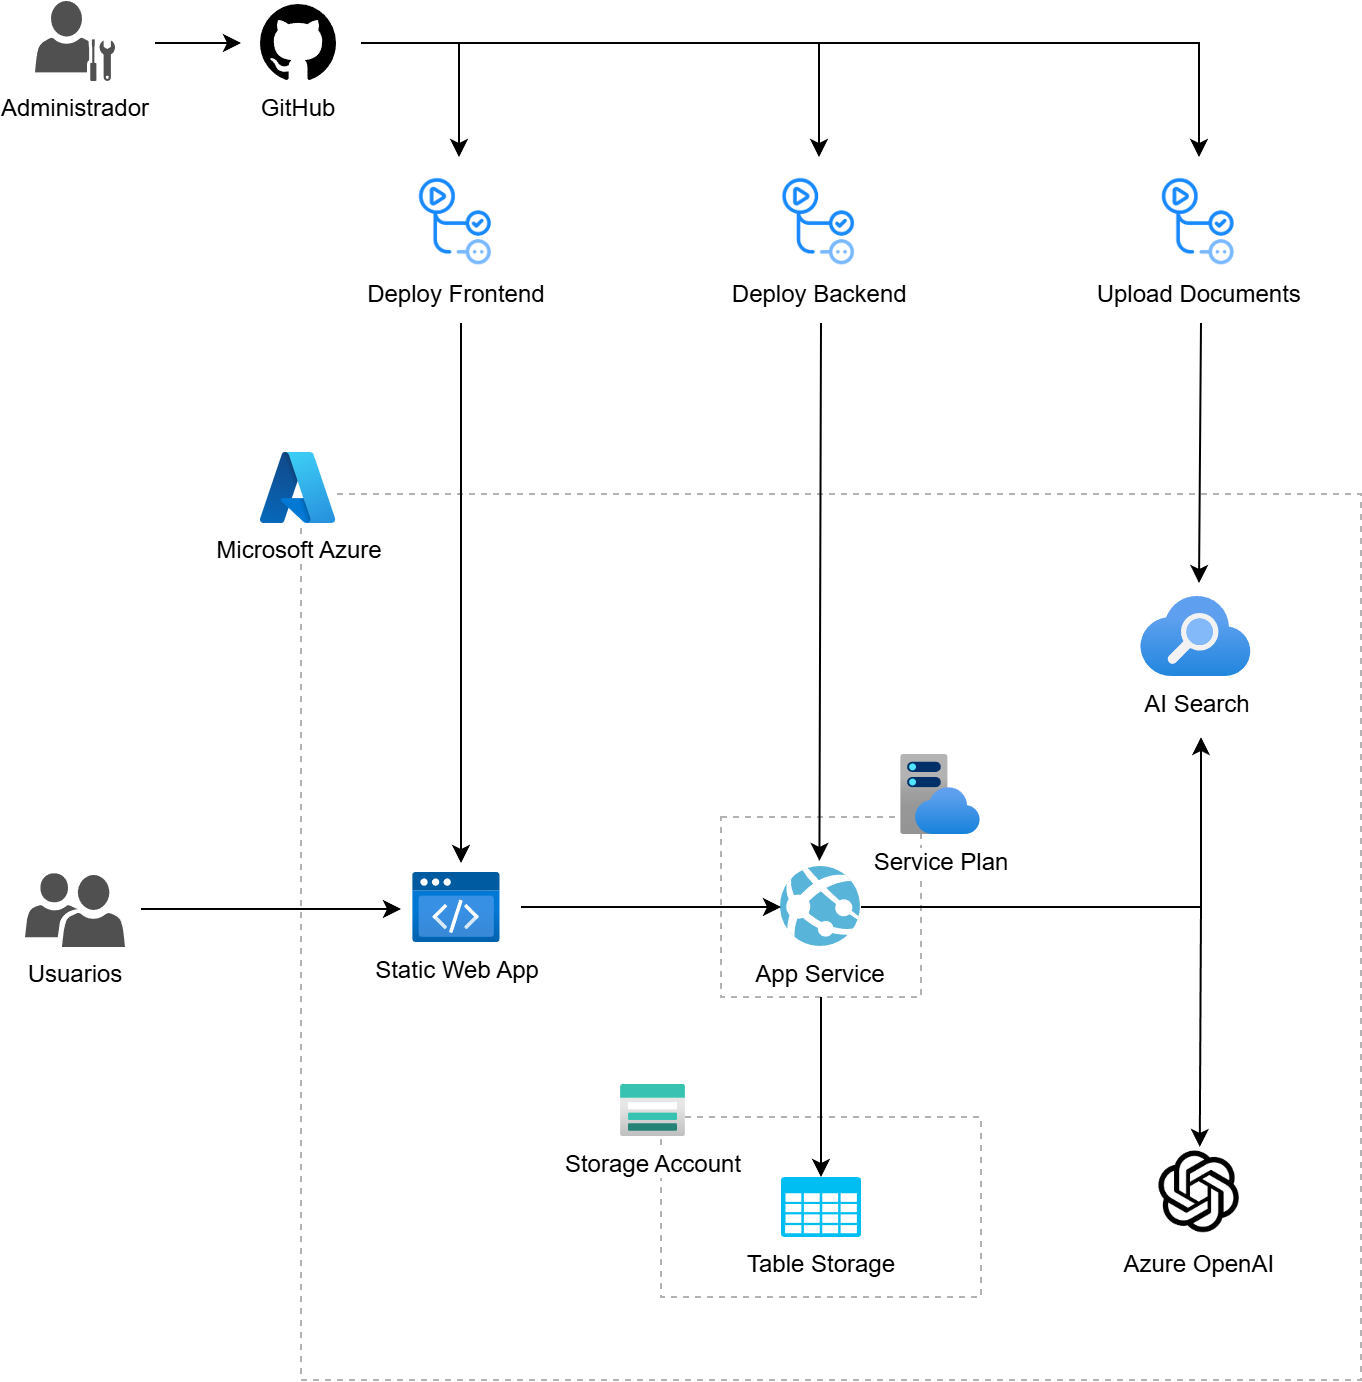
\includegraphics[scale=.55]{./Figures/arquitectura.png}
	\caption{Diagrama de arquitectura del sistema.}
	\label{fig:architecture}
\end{figure}

\vspace{8mm}

%---------------------------------------------------------------------------------------
\section{Configuración de la infraestructura en la nube}

Para garantizar el despliegue, disponibilidad y escalabilidad del sistema, se configuró una infraestructura en la nube basada en Microsoft Azure. 
A continuación, se describen los pasos principales para la configuración de cada recurso empleado en el proyecto.

\subsection{OpenAI Service}

El servicio de Azure OpenAI proporciona acceso a los potentes modelos de lenguaje de OpenAI, incluidos los más recientes. 
Estos modelos pueden adaptarse fácilmente a tareas específicas, como en este caso es la generación de contenido.

En la tabla \ref{tab:config-openai} se presenta un resumen de las configuraciones realizadas. 
Se seleccionó \textit{East US} como región, junto con el modelo de precios \textit{Standard S0}, 
adecuado para balancear el costo y el rendimiento del sistema.

Como medida de seguridad, se configuraron reglas de red para restringir el acceso únicamente al rango 
de direcciones IP del backend alojado en Azure App Service. Esto asegura que solo las solicitudes provenientes de la 
aplicación puedan acceder al modelo de lenguaje, lo que protege el servicio de accesos no autorizados.

Una vez desplegado el recurso, fue necesario seleccionar y desplegar los modelos específicos requeridos por el chatbot. 
En este caso, se optó por los siguientes modelos:

\begin{itemize}
	\item \textit{GPT-4o} como modelo de lenguaje para generación de respuestas. Este modelo está diseñado para brindar velocidad 
  y eficiencia, iguala la inteligencia de su antecesor \textit{GPT-4 Turbo}, y es notablemente más eficiente al entregar texto al 
  doble de velocidad y a la mitad del costo. Además, exhibe el rendimiento más alto en idiomas distintos del inglés en comparación 
  con los modelos de OpenAI anteriores.
	\item \textit{Ada-002} para el cálculo de \textit{embeddings} de texto. Este modelo supera a todos los modelos de \textit{embeddings} 
  anteriores en tareas de búsqueda de texto y similitud de oraciones.
\end{itemize}

Adicionalmente, es fundamental obtener el \textit{endpoint} y la \textit{key} del servicio, valores que se utilizan luego para la comunicación programática 
con Azure OpenAI. Estos datos se almacenan en el backend como variables de entorno para que el sistema pueda acceder al servicio de manera segura.

\begin{table}[h]
	\centering
	\caption[Configuración de Azure OpenAI]{Configuración de Azure OpenAI}
	\begin{tabular}{l l}    
		\toprule
		\textbf{Configuración} 	 & \textbf{Detalles} 	\\
		\midrule
		Región              &	East US 				        \\		
		Nivel de precios    & Standard S0				      \\
		Reglas de firewall  & Rango IP de App Service \\
    Modelos desplegados	& - gpt-4o				          \\
            	          & - text-embeddings-ada-002	\\
    Credenciales	      & Endpoint y Key 		      \\
		\bottomrule
		\hline
	\end{tabular}
	\label{tab:config-openai}
\end{table}

\subsection{AI Search}

Azure AI Search es un servicio de búsqueda en la nube con capacidades de inteligencia artificial integradas 
que enriquecen todo tipo de información con el fin de identificar y explorar fácilmente contenido relevante a escala.

La tabla \ref{tab:config-ai-search} presenta un resumen de las configuraciones realizadas. Se seleccionó la región de \textit{East US} y un nivel de precios 
\textit{Standard}, que ofrece hasta 50 índices para el almacenamiento y la búsqueda de documentos. En cuanto a la escala, el servicio se configuró para 
utilizar una sola unidad de búsqueda, lo cual es adecuado en principio para el volumen de consultas esperado y los requisitos de rendimiento.

Al igual que con el servicio de Azure OpenAI, se configuraron reglas de red restrictivas para mejorar la seguridad del servicio, al permitir 
únicamente el acceso desde el rango de direcciones IP asociado al backend. 

Aquí también es fundamental obtener la \textit{key} y la \textit{URI} del servicio para integrarlos en las variables de entorno del backend.

Es importante destacar que no es necesario crear un índice manualmente en esta etapa, ya que este será generado automáticamente como parte del pipeline de despliegue.

\begin{table}[h]
	\centering
	\caption[Configuración de Azure AI Search]{Configuración de Azure AI Search}
	\begin{tabular}{l l}    
		\toprule
		\textbf{Configuración} 	 & \textbf{Detalles} 	\\
		\midrule
		Región              &	East US 				        \\		
		Nivel de precios    & Standard				      \\
		Reglas de firewall  & Rango IP de App Service \\
    	Credenciales	      & URI y Key 		      \\
		\bottomrule
		\hline
	\end{tabular}
	\label{tab:config-ai-search}
\end{table}

\subsection{App Service}

En esta plataforma completamente administrada, uno puede alojar una aplicación avanzada en la nube sin necesidad de administrar la infraestructura.

Para alojar el backend del chatbot, se configura un App Service Plan con el SKU Basic B3, el cual proporciona 4 vCPU, 7 GB de RAM, 10 GB de almacenamiento remoto, y permite escalar hasta 3 instancias en caso de ser necesario. Como entorno de ejecución, se selecciona Python 3.10, y la región elegida es East US. Para optimizar los costos, se deshabilita la opción de zone redundancy.

Para que la aplicación funcione correctamente, es esencial configurar varias variables de entorno en el App Service. Estas variables incluyen las claves y los puntos de conexión de los servicios de Azure que se utilizan, así como los nombres de índices y modelos específicos. La siguiente tabla muestra las variables de entorno requeridas:

\begin{table}[h]
	\centering
	\caption[Configuración de Azure OpenAI]{Configuración de Azure OpenAI}
	\begin{tabular}{l c}    
		\toprule
		\textbf{Configuración} 	 & \textbf{Detalles} 	\\
		\midrule
		Región              &	East US 				        \\		
		Nivel de precios    & Standard S0				      \\
		Reglas de Firewall  & Rango IP de App Service \\
    Modelos desplegados	& gpt-4o				          \\
            	          & text-embeddings-ada-002	\\
    Credenciales	      & Endpoint y Key 		      \\
		\bottomrule
		\hline
	\end{tabular}
	\label{tab:config-openai}
\end{table}

Variable de Entorno	Descripción
AZURE OPENAI API KEY	Clave de acceso para el servicio de Azure OpenAI
AZURE OPENAI ENDPOINT	Endpoint del servicio de Azure OpenAI
AZURE SEARCH KEY	Clave de acceso para el servicio de Azure AI Search
AZURE SEARCH URI	URI del servicio de Azure AI Search
AZURE STORAGE CONNECTION STRING	Cadena de conexión para el almacenamiento de Azure
DB INDEX	Índice de la base de datos a utilizar
EMBEDDINGS MODEL	Modelo de embeddings a utilizar para el procesamiento

Para asegurar un monitoreo efectivo de la aplicación, se habilita la integración con Application Insights, permitiendo un seguimiento detallado de las métricas de rendimiento y uso. Adicionalmente, se activa la opción de Application Logging, de modo que los logs de la aplicación puedan ser visualizados directamente desde la terminal del App Service, facilitando la depuración y la supervisión continua.

Esta tabla resume la configuración principal del App Service, destacando los recursos asignados, las configuraciones de seguridad y monitoreo, así como los elementos clave necesarios para su correcta operación en el entorno de Azure.

\begin{table}[h]
	\centering
	\caption[Configuración de Azure OpenAI]{Configuración de Azure OpenAI}
	\begin{tabular}{l c}    
		\toprule
		\textbf{Configuración} 	 & \textbf{Detalles} 	\\
		\midrule
		Región              &	East US 				        \\		
		Nivel de precios    & Standard S0				      \\
		Reglas de Firewall  & Rango IP de App Service \\
    Modelos desplegados	& gpt-4o				          \\
            	          & text-embeddings-ada-002	\\
    Credenciales	      & Endpoint y Key 		      \\
		\bottomrule
		\hline
	\end{tabular}
	\label{tab:config-openai}
\end{table}

Configuración	Detalles
SKU del App Service Plan	Basic B3
Recursos del Plan	4 vCPU, 7 GB RAM, 10 GB de almacenamiento remoto
Escalabilidad	Hasta 3 instancias
Runtime	Python 3.10
Región	East US
Zone Redundancy	Deshabilitada
Monitoreo	Integración con Application Insights
Logging	Application Logging habilitado

\subsection{Static Web App}

Con Static Web Apps, el contenido estático como HTML, CSS y JavaScript e imágenes, se distribuye globalmente desde puntos de todo el mundo en lugar de un servidor web tradicional, por lo que los archivos están más cerca de los usuarios finales.

El recurso de Static Web App en Azure es sencillo de configurar, ya que solo requiere seleccionar un SKU y una forma de despliegue. En este caso, se ha optado por el SKU Standard, que proporciona características adicionales y soporte global. Como método de despliegue, se utiliza GitHub, lo cual permite una integración directa con el repositorio y facilita el control de versiones y el despliegue continuo de la aplicación.

A diferencia de otros servicios en Azure, las Static Web Apps se despliegan globalmente, por lo que no es necesario especificar una región. Además, no se requieren variables de entorno para este recurso, ya que todas las conexiones a otros servicios (como el backend y las APIs) son manejadas exclusivamente por el backend, simplificando la configuración.

Es importante obtener el deployment token de la Static Web App, ya que este token será necesario más adelante para configurar el pipeline de despliegue automático, permitiendo la autenticación y el despliegue seguro desde GitHub.

Configuración	Detalles
SKU	Standard
Método de Despliegue	GitHub
Región	Despliegue global
Variables de Entorno	No aplicable
Token de Despliegue	Requerido para configurar el pipeline

Esta tabla resume los aspectos clave de la Static Web App

\subsection{Table Storage}

Para implementar el recurso de Table Storage, primero se desplegó una Storage Account en la región East US, manteniendo la consistencia con los demás recursos del sistema. Se seleccionó Tables como servicio principal y se configuró una performance de tipo Standard, adecuada para las necesidades de la aplicación.

En cuanto a la redundancia de los datos, se eligió la opción de Almacenamiento Localmente Redundante (Locally-redundant storage), una alternativa rentable que asegura que los datos estén replicados dentro de un único centro de datos en la misma región, reduciendo costos sin comprometer la disponibilidad básica.

Una vez que la cuenta de almacenamiento fue desplegada, se procedió a crear la tabla FeedbackTable, que servirá para almacenar los comentarios y opiniones de los usuarios recopilados a través del sistema. Es importante obtener la connection string de la Storage Account, ya que será necesaria para conectar la aplicación con esta tabla y permitir el acceso programático.

Configuración	Detalles
Región	East US
Servicio Principal	Tables
Performance	Standard
Redundancia	Locally-redundant storage
Nombre de la Tabla	FeedbackTable
Connection String	Necesaria para conectar la aplicación

Esta tabla resume los aspectos clave de la configuración de Table Storage

%---------------------------------------------------------------------------------------
\section{Procesamiento de los documentos}

%---------------------------------------------------------------------------------------
\section{Lógica de comunicación entre el usuario y el modelo}

%---------------------------------------------------------------------------------------
\section{API}

%---------------------------------------------------------------------------------------
\section{Interfaz de usuario}

%---------------------------------------------------------------------------------------
\section{Pipelines de despliegue automático}